\documentclass[tikz, border=10pt, ]{standalone}

\usetikzlibrary{arrows}

\begin{document}
	
	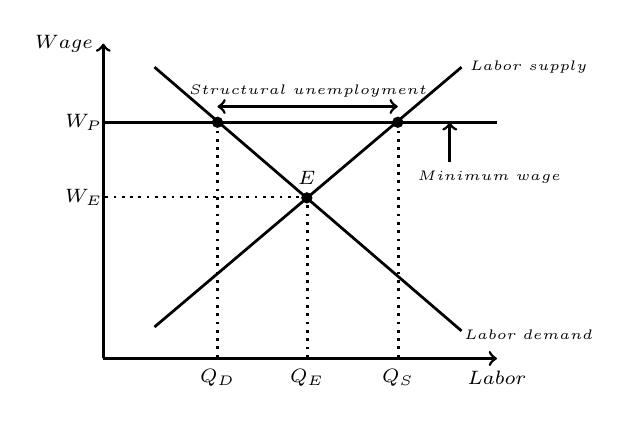
\begin{tikzpicture}[line width=1pt]
		\draw[->] (0, 0) -- (5, 0); % Горизонтальная линия
		\draw[->] (0, 0) -- (0, 4); % Вертикальная линия
		
		\draw (0, 3) -- (5, 3);
		
		\draw (0.65, 3.7) -- (4.55, 0.35);
		\draw (0.65, 0.4) -- (4.55, 3.7);
		
		\draw[dotted] (1.45, 3) -- (1.45, 0);
		\draw[dotted] (3.75, 3) -- (3.75, 0);
		
		\draw[dotted] (2.59, 2.05)-- (2.59, 0);
		\draw[dotted] (2.59, 2.05)-- (0, 2.05);
		
		\draw[<->] (1.45, 3.2)-- (3.74, 3.2);
		
		\draw[->] (4.4, 2.5) -- (4.4, 3);
	\begin{scriptsize}
		\draw[fill=black] (1.45, 3) circle (1.5pt);
		\draw[fill=black] (3.74, 3) circle (1.5pt);
		\draw[fill=black] (2.585, 2.04) circle (1.5pt);
		
		\draw (-0.5, 4) node {$Wage$};
		\draw (5, -0.25) node {$Labor$};
		
		\draw (-0.25, 3) node {$W_P$};
		\draw (-0.25, 2.05) node {$W_E$};
		
		\draw (2.585, 2.3) node {$E$};
		
		\draw (1.45, -0.25) node {$Q_D$};
		\draw (2.585, -0.25) node {$Q_E$};
		\draw (3.74, -0.25) node {$Q_S$};
		
		\tiny
		\draw (2.6, 3.4) node {$Structural~unemployment$};
		\draw (5.4, 0.3) node {$Labor~demand$};
		\draw (5.4, 3.7) node {$Labor~supply$};
		\draw (4.9, 2.3) node {$Minimum~wage$};
	\end{scriptsize}
\end{tikzpicture}
\end{document}